\chapter{Zeit: Takt, Uhrwerk und lesbare Veränderung}
\label{ch:zeit}
\section{Drei Bedeutungen des Wortes Clock}
Eine zyklische Matrix ist zunächst ein Taktmuster. Eine Dynamik sagt, wann welcher Zustand entsteht. Eine Uhr braucht zusätzlich eine beobachtbare Anzeige und eine Kalibrierung. Diese drei Ebenen müssen zusammenpassen.

Die Familienoperation $\sigma$ besitzt Ordnung drei. Ein markierter Lift $c=i\sigma$ erfüllt $c^4=\sigma$ und $c^{12}=I$. Auf Observablen verschwindet die globale Phase $i$ bei der Konjugation; ihre Periode ist dann höchstens drei. Die Ordnung zwölf kann nur relativ zu einer Phasenreferenz sichtbar werden.

Für ein unitäres $A$ gilt am Singulett
\begin{equation}
A^{\otimes4}\Omega=\det(A)\Omega,
\quad\bra\Omega A_1\ket\Omega=\frac{\Tr A}{4},
\quad p_{1j}=\frac{16-|\Tr A|^2}{24}.
\end{equation}
Bei nichtunitären Filtern müssten Normierung und Erfolgswahrscheinlichkeit ergänzt werden. Für den ausgewählten Dreierzyklus ist $|\Tr c|=1$; die Paarenergien sind $5/8$ und die Gesamtenergie $15J/8$ außerhalb der Rückkehrschritte. Die Paartests sehen Periode drei, der phasentreue Überlapp des Lifts Periode zwölf. \src{S08, §4; S01, §5}

\section{Warum die Paarenergien unter dem Tetramer stillstehen}
Der vollständige gleichgewichtete Tetramer-Hamiltonoperator ist eine zentrale Transpositionssumme. Deshalb kommutiert er mit jedem $S_{ij}$ und jedem $P^+_{ij}$. Die Paarenergien ändern sich unter seiner freien Entwicklung nicht. Eine Tabelle, die nacheinander einen lokalen $c$-Tick anwendet, ist somit kein Beweis, dass genau diese Anzeige unter $H_{\mathrm{tet}}$ von selbst läuft.

Auch der bedingte Dreiträgersektor $\Lambda^3\C^4\cong\overline4$ bildet eine einzige irreduzible $\mathrm{SU}(4)$-Darstellung. Ein vollständig $\mathrm{SU}(4)$-invarianter Systemgenerator wirkt dort nach Schurs Lemma skalar. Zusätzliche invariant gebaute Terme spalten die vier bedingten Lesarten nicht einfach auf. Das ist die stärkere Form des in S07 zunächst über drei Energieniveaus beschriebenen Hindernisses.

\section{Eine laufende lokale Anzeige im gesetzten Modell}
Ein präparierter nichtstationärer Zustand kann dennoch unter demselben Tetramer laufen. Für einen lokalen spurfreien hermiteschen Pauli $A$ mit $A^2=I$ setze
\begin{equation}
\ket{\psi(0)}=e^{-i\pi A_1/4}\Omega
=\frac{\Omega-iA_1\Omega}{\sqrt2}.
\end{equation}
Da $H_{\mathrm{tet}}A_1\Omega=2JA_1\Omega$, folgt
\begin{equation}
\langle A_1\rangle_t=-\sin(2Jt/\hbar),\qquad
\langle A_j\rangle_t=\tfrac13\sin(2Jt/\hbar)\quad(j\ne1).
\end{equation}
Die lokalen Anzeigen oszillieren gegeneinander; ihre Summe bleibt null. Die Periode ist $\pi\hbar/J$. Präparation, Ausleserichtung und die Kalibrierung von $J$ sind weitere Eingaben. \src{S01, §5.2}

\begin{figure}[H]\centering
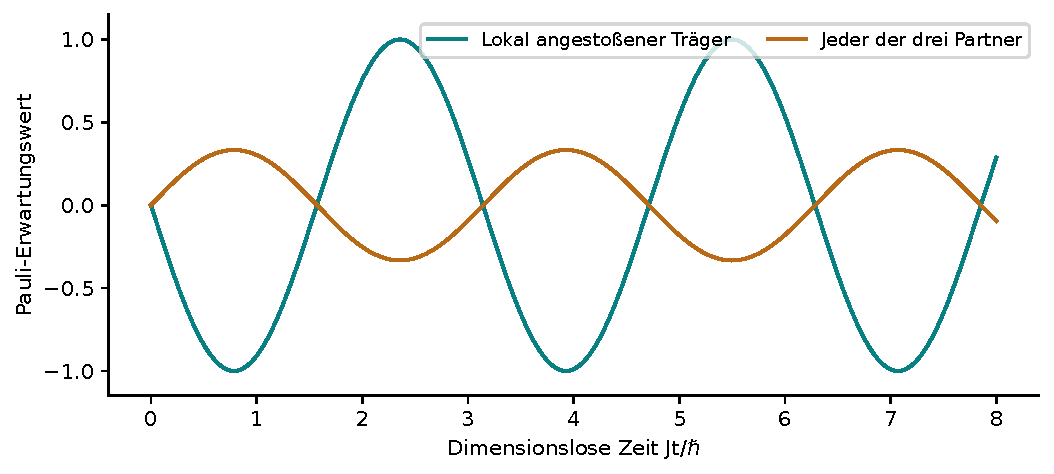
\includegraphics[width=.94\linewidth]{figures/clock.pdf}
\caption{Ein lesbares Uhrsignal trotz konstanter Paarenergien. Unterschiedliche Observablen beantworten unterschiedliche Fragen.}
\end{figure}

\section{Eine relationale Viereruhr ist konstruierbar}
Zerlege $\Omega=\frac12\sum_{a=0}^3\ket a_C\ket{\omega_a}_S$. Die vier $\omega_a$ sind orthonormal. Wähle zusätzlich
\begin{equation}
h=\frac{\hbar\omega}{2}\operatorname{diag}(-3,-1,1,3),\quad
H_C=h_0,\quad H_S=h_1+h_2+h_3.
\end{equation}
Weil jedes Wort von $\Omega$ jedes Energielabel einmal enthält, gilt $(H_C+H_S)\Omega=0$. Für
\begin{equation}
\ket t_C=\frac12\sum_a e^{-i\epsilon_at/\hbar}\ket a,
\qquad \ket{\psi(t)}_S=2\,{}_C\bra t\Omega\rangle
\end{equation}
erhält man $\psi(t)=e^{-iH_St/\hbar}\psi(0)$. Die Zeiten $t_k=k\pi/(2\omega)$ liefern vier orthogonale Anzeigen. Global ist der Zustand stationär, bedingt auf die Uhranzeige entwickelt sich das System. Das ist eine konkrete Page-Wootters-Konstruktion, aber mit zusätzlich gewählter Basis, Energieleiter und Fourierauslesung. \src{S01, §5.4; S05, §8; S06}

Eine rein diskrete Alternative aus S05 verwendet den Viererzyklus $R\ket j=\ket{j+1\bmod4}$. In der Zweiqubitkodierung lässt er sich aus CNOT und Pauli-$X$ bauen. Mit $U_C=R$ und $U_S=-R^{\otimes3}$ gilt
\begin{equation}
(U_C\otimes U_S)\Omega=\Omega,\qquad U_S\omega_a=\omega_{a+1}.
\end{equation}
Dieser Tick ist nicht der ausgezeichnete Familienzyklus. Die Existenz einer Uhr ist damit konkret; ihre eindeutige Quellauswahl bleibt offen. Eine experimentelle Illustration des allgemeinen relationalen Zeitgedankens findet sich bei \href{https://arxiv.org/abs/1310.4691}{Moreva et al. [E3]}.

\section{Warum ein Logarithmus noch keine Sekunde ist}
Aus $\lambda^n=e^{-n\delta}$ folgt $\delta=-\log\lambda$. Die historischen Größen $6\log(3/2)$ und $6\log3$ beschreiben deshalb sechsfach wiederholte Faktoren $(2/3)^6$ und $(1/3)^6$. Eine physikalische Rate ist erst $\delta/\tau$ für einen festgelegten Schritt $\tau$.

Eine dimensionslose Theorie muss keinen menschlichen Meter oder eine Sekunde absolut auswählen. Sie muss jedoch die beobachtbaren Verhältnisse und eine konsistente Relation ihrer Skalen bestimmen. Der Vermittlungsansatz lokalisiert die Energieskala auf $t^2/\Delta$, leitet aber weder $t$ noch $\Delta$ aus der algebraischen Struktur allein her.

\chapter{Die ausführbare Präparation und der Mehrzeittest}
\label{ch:echo}
\section{Was S02 tatsächlich geschlossen hat}
Die Präparationsnotiz S02 geht über den abstrakten Satz „$\Omega$ existiert“ hinaus. Sie beschreibt eine konkrete Schaltung, die aus einem einfachen Eingang den Zustand mit Erfolgsanzeige herstellt, anschließend ein Register schreibt und die Rückkehr ausliest. Laut Quelle wurde die Schaltung exakt simuliert, nicht auf Hardware ausgeführt. Ihr Zugriff auf zusätzliche Hilfssysteme und Nicht-Clifford-Operationen ist ausdrücklich angenommen.

Die gemeinsame Wechselwirkung ist der kohärent kontrollierte Swap
\begin{equation}
F_{R;ij}=\ket0\bra0_R\otimes I+\ket1\bra1_R\otimes S_{ij}.
\end{equation}
Ein passender Generator ist
\begin{equation}
H_{\mathrm{int}}=\hbar g\ket1\bra1_R\otimes P^-_{ij},\quad
g\tau=\pi\quad\Longrightarrow\quad e^{-iH_{\mathrm{int}}\tau/\hbar}=F_{R;ij}.
\end{equation}
Der Beweis nutzt nur die Projektoreigenschaft $G^2=G$: $e^{-i\pi G}=I-2G$.

Die Swap-Identität $S=\frac14\sum_{v=0}^{15}P_v\otimes P_v$ zeigt, wie der Generator im Quell-Pauli-Raum liegt:
\begin{equation}
G=\frac3{16}(I-Z_R)\otimes I
-\frac1{16}\sum_{v=1}^{15}I_R\otimes P_v\otimes P_v
+\frac1{16}\sum_{v=1}^{15}Z_R\otimes P_v\otimes P_v.
\end{equation}
Die Terme kommutieren. Die algebraische Schreibbarkeit ist genau; physische Adressierbarkeit, Pulsfläche, Reset und Messbarkeit folgen daraus noch nicht.

\section{Die zusätzliche Ressource bleibt sichtbar}
Der benötigte Zustand $\Omega$ ist in der Acht-Qubit-Kodierung kein Stabilizerzustand. Schon für einen nichttrivialen lokalen Pauli gilt
\begin{equation}
\langle P^{(i)}P^{(j)}\rangle_\Omega=-\frac13,
\end{equation}
während reine Qubit-Stabilizerzustände für Pauli-Observablen nur $0,\pm1$ liefern. Ebenso ist der Paarreduktionsrang sechs keine Zweierpotenz. Eine exakte Präparation aus einem Stabilizer-Eingang benötigt deshalb eine zusätzliche Ressource, etwa einen passenden Nicht-Clifford-Zugriff. Kontinuierlicher Austausch kann die Cliffordklasse verlassen, beseitigt aber allein nicht die genannte Singulett-Erhaltungsgröße.

Eine kontrollierte Qubitvertauschung besitzt die Folge
\begin{equation}
\mathrm{CX}(a,b);\quad \mathrm{CCX}(R,b,a);\quad\mathrm{CX}(a,b).
\end{equation}
Zwei solche Fredkin-Bausteine vertauschen zwei Ququarts. Der Toffoli-Teil ist nicht Clifford. S02 löst ihn in Clifford- und sieben $T/T^\dagger$-Gatter auf, mit $T=\operatorname{diag}(1,e^{i\pi/4})$. Diese Sieben ist eine transparente Kostenobergrenze der dort gewählten Zerlegung, keine behauptete globale Minimalität.

Ein Nicht-Stabilizer-Hilfszustand oder ein entsprechender Nicht-Clifford-Puls kann die fehlende Ressource liefern. Ihre allgemeine Rolle in der Quantenrechnung ist bekannt. Ihre physikalische Herkunft aus TFPT ist eine andere Frage. \href{https://arxiv.org/abs/quant-ph/0403025}{Bravyi und Kitaev [E4]}

\section{Wie der Filter den Zustand erzeugt}
Der einfache Eingang lautet
\begin{equation}
\chi_0=\frac{\ket{01}-\ket{10}}{\sqrt2}
\otimes\frac{\ket{23}-\ket{32}}{\sqrt2}.
\end{equation}
Er ist mit dem in S02 angenommenen Clifford-Baukasten präparierbar und besitzt $\Omega$-Anteil $1/6$. Der Antisymmetrisierer ist
\begin{equation}
A_4=\ket\Omega\bra\Omega
=\frac1{24}\sum_{\pi\in S_4}\operatorname{sgn}(\pi)U_\pi.
\end{equation}
Die konkrete Schaltung erzeugt 32 Kontrollzweige, von denen 24 die Permutationen tragen. Acht ungültige Zweige werden markiert. Nach Interferenz und Erfolgsselektion ist der implementierte Operator
\begin{equation}
K_{\mathrm{prep}}=\frac1{32}\sum_{\pi\in S_4}\operatorname{sgn}(\pi)U_\pi
=\frac34A_4.
\end{equation}
Somit gilt
\begin{equation}
p_{\mathrm{prep}}=\frac9{16}\frac16=\frac3{32}=9{,}375\%.
\end{equation}
Der erfolgreiche Zweig ist exakt $\Omega$. Die restlichen $29/32$ Versuche sind Misserfolge und dürfen nicht unsichtbar werden. Bei unabhängigen Neuansätzen benötigt man im Mittel $32/3$ Versuche. Das ist eine heraldierte Präparation, kein deterministischer Kühlmechanismus.

\section{Das ursprüngliche Echo: eins gegen siebzehn Zweiunddreißigstel}
Für $S=S_{01}$ schreibe $V=H_RF_{R;01}H_R$. Dann
\begin{equation}
V(\ket0_R\otimes\psi)=\ket0_R\otimes P_+\psi+\ket1_R\otimes P_-\psi,
\quad V^2=I.
\end{equation}
Ein ignorierter frischer Pointer erzeugt
\begin{equation}
\Delta_S(\rho)=\tfrac12(\rho+S\rho S),\qquad\Delta_S^2=\Delta_S.
\end{equation}
Diese \emph{binäre Swap-Aufzeichnung} ist ein anderer Kanal als die 15-Kontext-Mischung mit Faktor $3/7$.

Vor der Aufzeichnung wird auf einem Träger ein lokaler Dreierzyklus $c$ mit $c^3=I$ und $\Tr c=1$ angewendet. Ohne diesen Tick wäre $\Omega$ bereits Swap-Eigenzustand und beide Ausführungen wären für den Test gleich. Danach folgen zwei Anwendungen von $V$, Rücknahme von $c$ und der gleiche Endfilter wie bei der Präparation. Es gilt
\begin{equation}
\langle c_0\Omega|S_{01}|c_0\Omega\rangle=\frac14,
\quad p_+=\frac58,\quad p_-=\frac38.
\end{equation}
Mit demselben kohärenten Pointer hebt die zweite Anwendung die erste auf. Mit frischen Pointern bleibt die Dephasierung. Der normierte Rückkehrwert ist daher
\begin{equation}
F_{\mathrm{behalten}}=1,\qquad
F_{\mathrm{frisch}}=p_+^2+p_-^2=\frac{17}{32}.
\label{eq:originalecho}
\end{equation}

\begin{figure}[H]\centering
\begin{tikzpicture}[node distance=8mm]
\node[box,text width=25mm] (p) at (0,0) {$\Omega$ erfolgreich\\präpariert};
\node[box,text width=19mm] (c) at (3,0) {Lokaler\\Tick};
\node[box,text width=35mm] (r) at (6.8,.9) {$V$, dann $V$\\gleicher Pointer};
\node[openbox,text width=35mm] (f) at (6.8,-1) {$V$, dann $V$\\frische Pointer};
\node[box,text width=24mm] (e) at (10.8,0) {Tick zurück\\Endfilter};
\draw[arr] (p)--(c);\draw[arr] (c)--(r);\draw[arr] (c)--(f);
\draw[arr] (r)--(e);\draw[arr] (f)--(e);
\end{tikzpicture}
\caption{Die Zweige stimmen nach der ersten reduzierten Aufzeichnung überein. Erst die Fortsetzung unterscheidet, ob die erste Aufzeichnung kohärent verfügbar bleibt.}
\end{figure}

\section{Die wirklichen Erfolgswahrscheinlichkeiten}
Der Endfilter hat den Effekt $K_{\mathrm{prep}}^\dagger K_{\mathrm{prep}}=(9/16)A_4$. Seine beobachtbare Erfolgsrate ist deshalb $(9/16)F$, nicht $F$ selbst.
\par\noindent\begin{tabularx}{\linewidth}{L{68mm}Y Y}
\toprule
\textbf{Statistik}&\textbf{Behalten}&\textbf{Frisch}\\\midrule
$\Omega$-Rückkehr, bedingt auf Präparation&$1$&$17/32$\\
Endfilter erfolgreich, bedingt auf Präparation&$9/16$&$153/512$\\
Beide Filter erfolgreich, je begonnenem Versuch&$27/512$&$459/16384$\\
Alle übrigen Ausgänge&$485/512$&$15925/16384$\\\bottomrule
\end{tabularx}\par
Die gemeinsamen Erfolgsraten sind etwa $5{,}2734\%$ und $2{,}8015\%$. Ein hoher bedingter Rückkehrwert ist also keine hohe Gesamtausbeute.

Nach $n$ Aufzeichnungen mit demselben Pointer alterniert $F$ zwischen eins für gerade $n$ und $17/32$ für ungerade $n$. Bei frischen Pointern bleibt es ab $n=1$ bei $17/32$. Alle einzelnen Träger bleiben dabei maximal gemischt. Die unterscheidende Information sitzt in zugänglichen Korrelationen.

Bei Pointerdephasierung mit verbleibender Kohärenz $0\le\eta\le1$ ergibt das in S02 festgelegte Modell
\begin{equation}
F(\eta)=\frac{17+15\eta}{32}.
\end{equation}
Vollständige Dephasierung zerstört das Echo; ohne Tick liefern beide Zweige eins. Ein reiner Pointer-$Z$-Fehler ergibt $F=1/16$. Die Quelle beschreibt zudem Negativkontrollen ohne Permutationsvorzeichen, ohne Aufzeichnungs-Swaps und mit fälschlich wiederverwendetem Pointer.

\section{Neue Fortsetzung: der maximal ausgeglichene Echovergleich}
\status{Eigene exakte Ergänzung dieser Synthese.} Man kann die gleiche Messfrage für einen beliebigen lokalen unitären Tick $A$ ausrechnen. Setze
\begin{equation}
s=\langle A_0\Omega|S_{01}|A_0\Omega\rangle
=\frac{4-|\Tr A|^2}{12}.
\end{equation}
Die beiden Swap-Gewichte sind $(1\pm s)/2$. Daher
\begin{equation}
F_{\mathrm{frisch}}=\frac{1+s^2}{2},\qquad
F_{\mathrm{behalten}}-F_{\mathrm{frisch}}=\frac{1-s^2}{2}\le\frac12.
\label{eq:optimal}
\end{equation}
Der Kontrast dieser Rückkehrstatistik ist maximal, wenn $s=0$, also $|\Tr A|^2=4$. Ein einzelnes CNOT innerhalb des Viererträgers erfüllt $\Tr A=2$. Es permutiert dieselbe Menge von 60 Stabilizerprojektoren. Damit liefert der vorhandene lokale Tick-Baukasten die klarere Variante
\begin{equation}
\boxed{F_{\mathrm{behalten}}=1,\qquad F_{\mathrm{frisch}}=\frac12.}
\end{equation}
Mit denselben Filterfaktoren sind die gemeinsamen Rohwahrscheinlichkeiten $27/512$ und $27/1024$. Das Dephasierungsmodell vereinfacht sich zu $F(\eta)=(1+\eta)/2$.

Die neue Variante wurde auf dem expliziten ganzzahligen $\Omega$-Tensor und der vollständigen Standardprojektormenge nachgerechnet. Der gesamte ursprüngliche 20-Qubit-Schaltungsexport wurde hier nicht neu kompiliert. Die Aussage ist ein mathematisch konkreter Anschluss und keine nachträgliche Änderung des in S02 eingefrorenen Haupttests. „Maximal“ bezieht sich auf \eqref{eq:optimal}, also genau diese Rückkehrmessung mit einem lokalen Tick und binärer Swap-Dephasierung, nicht auf alle denkbaren Unterscheidungsprotokolle.

\begin{figure}[H]\centering
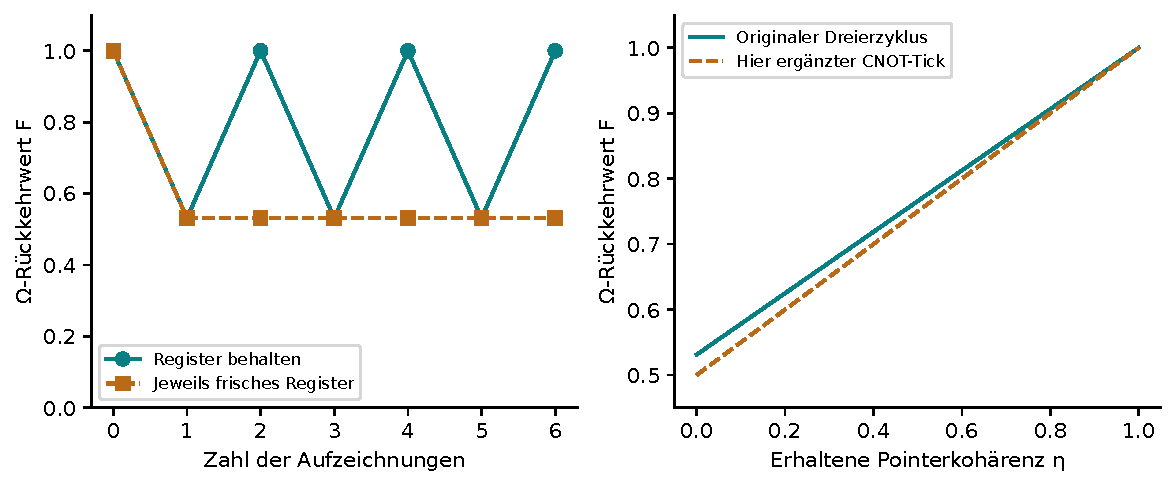
\includegraphics[width=\linewidth]{figures/echo.pdf}
\caption{Links das ursprüngliche Mehrzeitecho. Rechts die ursprüngliche und die neu ergänzte ausgeglichene Variante unter demselben vorgegebenen Pointer-Dephasierungsmodell. Es sind Vorhersagekurven, keine experimentellen Messpunkte.}
\end{figure}

Ein einfaches robustes Zertifikat verbindet die neue Variante mit der Zellprüfung: Falls $\bra\Omega\rho\ket\Omega\ge1-\varepsilon$, weicht jede der idealen Ausgangswahrscheinlichkeiten unter denselben fehlerfreien Folgekanälen um höchstens $\sqrt\varepsilon$ ab. Der Kontrast ist daher mindestens $1/2-2\sqrt\varepsilon$. Das ist eine konservative Schranke aus Spurdistanz und ihrer Kontraktivität, keine vollständige Hardwarefehleranalyse.

\section{Ressourcen und Beweisgrenze der Originalschaltung}
\par\noindent\begin{tabularx}{\linewidth}{Y r}
\toprule \textbf{Ressource nach S02}&\textbf{Anzahl}\\\midrule
Systemqubits&8\\Filterhilfsqubits, wiederverwendet&10\\Pointerplätze&2\\Insgesamt reservierte Qubits&20\\Klassische Erfolgsbits beider Filter&12\\Toffoli-Gatter&574\\Weitere CNOT vor Toffoliauflösung&382\\Hadamard&26\\Pauli-$X$ / Pauli-$Z$&276 / 26\\$T/T^\dagger$ in der gewählten Auflösung&4018\\\bottomrule
\end{tabularx}\par
Ein einzelner Filter verwendet 285 Toffolis. Routing, Fehlerkorrektur, reale Pulse und die Herstellung geeigneter Hilfszustände sind nicht enthalten. Laut S02 bestehen 598 benannte Bedingungen; normale und optimierte Ausführung sowie der unabhängige Paketlauf erzeugten identische Dateien. Die exportierten Hauptschaltungen wurden erneut aus ihren OpenQASM-Zeilen ausgeführt; die vollständigen Clifford+$T$-Varianten waren durch lokale Matrixidentität und Ersetzung zertifiziert, nicht zusätzlich als komplette komplexe 20-Qubit-Vektoren simuliert.

Die Vorhersagedatei wurde laut Quelle am 14. September um 05:51:45 UTC vor dem neuen Prüflauf fixiert. Das ist ein interner Simulationsvertrag mit analytischen Zielwerten, keine externe Studienregistrierung. Das Echo unterscheidet zwei konkrete Ergänzungen derselben ersten Schattenregel. Es identifiziert nicht allein einen einzigartigen Universalraum.
